\documentclass[conference]{IEEEtran}
\hyphenation{op-tical net-works semi-conduc-tor}

\usepackage{graphicx}

\begin{document}
\title{Freedom Fridays: Designing 100 Faulty Lightbulbs}

\author{
\IEEEauthorblockN{Dean Sutton}
\IEEEauthorblockA{ORGX}
}

% make the title area
\maketitle

\begin{abstract}
I propose creating a freedom system where people are free to explore, fail and
then succeed. The symbolic name for this system is \emph{Freedom Fridays}.
People get a day a week free from normal duties. This system will rely on
supporting leadership, training, and trust to overcome the problems that plague
parts of the organisation. Problems include purpose (a.k.a. task) switching,
fear of failure, and singular points of view.
\end{abstract}

\section{Introduction}
Providing the support for people to fail is key to company growth. Why? before
growth comes learning. Learning requires failure. Therefore, ORGX must
learn how to learn and deal with failure. This will involve training, but more
importantly it will require leadership that embraces failure as a sign of learning.

This following documents three key problems that are inhibiting growth and
proposes the first step towards overcoming the problems. Suggestions are made
for further steps and basic analysis of how these steps reinforce the first
step.

\section{The Key Problems}
Three key problems are inhibiting growth. They are purpose switching, fear of
failure, and singular points of view.

\subsection{Purpose Switching}
ORGX has multiple purposes. Different parts of the organisation deal with one
or maybe more of those purposes. Purpose switching sometimes gets mistaken for
task switching. Task switching is hard, but it gets harder when you also switch
purpose. People with really high emotional quotients can deal with this.
However, for the mere mortal it leads to confusion. Introverts, especially well
educated ones, don't like to be confused. Confusion in combination with pressure
to achieve results leads to amygdala hijacks and the inability to think
objectively. This is a negative cycle. Figure \ref{fig:peoplesystems} shows the
positive feedback cycle. People need to feel that they create and operate
systems that produce valuable things to affirm their purpose.

\begin{figure*}[!t]
\centering
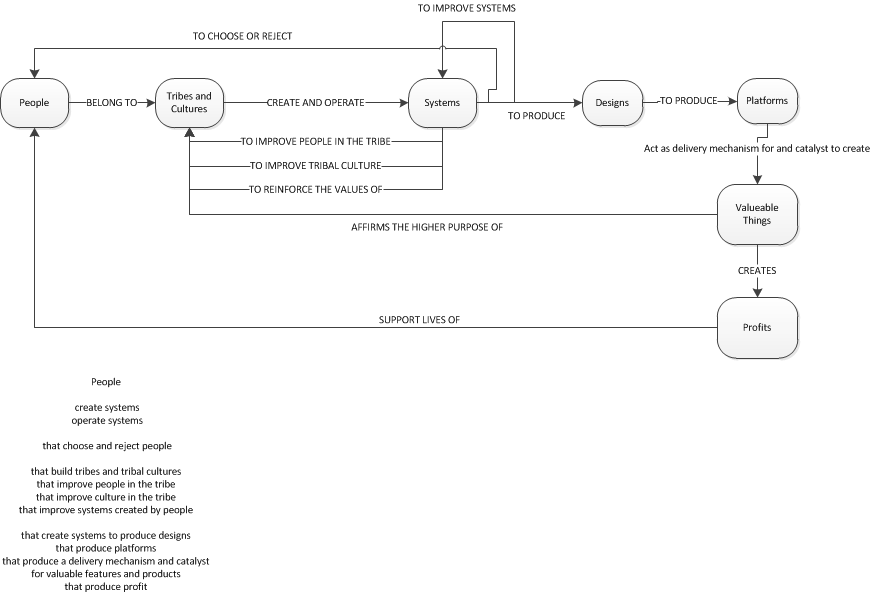
\includegraphics[width=\textwidth]{SystemCreation.png}
\caption{The positive feeback cycle between tribes, people, systems and company profit. \textcopyright Grant Reid}
\label{fig:peoplesystems}
\end{figure*}


\subsection{Fear of Fail}
When did I do my most learning. University. Why? I failed heaps.



\subsection{Singular Point of View}
Three objects on a table. A rugby ball, toilet paper and a gold golf ball. The
objective is to take the object of most value. However, two people are chosen to
decide what object to take. They both look at the objects from different
perspectives. One can see the golf ball, the other can not. How does the person
who sees the golf ball convince the other that it is there? This situation
usually leads to fighting when there is an absense of trust.

\section{Designing the Light Bulb}

\subsection{Freedom Fridays}

\subsubsection{Risks}
People spending more than there alloted amount. (This should be mitigated by
people behaving as professions. I.E. when work needs to be done they may use
their freedom time to do it.)

Middle managers place control over what people work on. (Mitigated by
leadership training PDLC - You have your people for 80 percent of time. Make
their time valuble)

People go cowboy with idea (start selling etc..) Mitigated by new technology
manager/team. 

\subsection{Next Steps}
Present a problem, present a solution - Any team

Emotional Intelligence course. Increase EQ. People need to be aware of their
amgdala hyjacks

Paradigm breaking - S-Curve, you don't have to build it to sell the idea.

Innovation pipeline. Need to come up with method so employees can turn their
free ideas (if they want to) into company products.

\section{Conclusion}
The conclusion goes here.

\end{document}

